\section{Méthode du point fixe}

\subsection{Principe de la méthode du point fixe}
Il est parfois possible de résoudre de manière itérative des équations de la forme $$g(x)=x$$

Les solutions de cette équation sont appelées les \guillemets{points fixes} de  $g$. Elles représentent les préimages qui sont invariantes par $g$ ou, de manière équivalente, les valeurs ou $g$ intersecte la fonction identité.

\medskip
Il est clair qu'il est toujours possible de ramener la recherche d'un zéro d'une fonction $f$ à la recherche d'un point fixe d'une fonction $g$; il suffit, par exemple, de poser $g(x)=f(x)+x$ et dans ce cas :
$$f(x)=0 \ssi[3] g(x)=x$$
Cependant et comme nous aurons l'occasion de le constater, bien que le fait de définir $g(x)=f(x)+x$ semble naturel, ce choix ne sera pas toujours le meilleur.


\medskip
\begin{minipage}[t][][b]{0.6\textwidth}
La \textit{méthode du point fixe} consiste à construire une suite $\left(x_{n}\right)_{n\in\N}$ définie par :
$$x_{n+1}=g(x_n) \eh{3}\textrm{et $x_0$ est choisit arbitrairement}$$

\medskip
Il est intéressant de comprendre à l'aide d'un graphique le mécanisme de convergence de cette suite. \\
Si la \guillemets{variation} de la fonction n'est pas trop importante autour d'un éventuel point fixe, alors nous obtenons une succession de valeur qui vont être \guillemets{attirée} par le point fixe.


 
\end{minipage}\hspace{5mm}\begin{minipage}[t][][b]{0.4\textwidth}
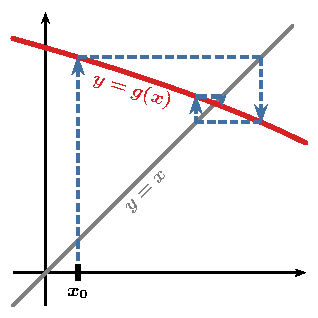
\includegraphics[scale=1]{Chapitre_3_analyse_numerique/figures/fig_9/fig_9.pdf}
\end{minipage}


%\medskip
%Cette méthode est motivée par la résultat du théorème \ref*{prop:point_fixe}, qui assure qu'en cas de convergence de cette suite, la valeur de convergence est un point fixe de la fonction $g$.
%
%\medskip
%\begin{proposition}
%\label{prop:point_fixe}
%Soit $g:[a;b]\rightarrow [a;b]$ une fonction continue et $x_0\in [a;b]$.\\
%Supposons que la suite $(x_n)_{n\ge0}$ définie comme ci-dessus converge vers $\ell$. Alors :
% 
%$$\ell=g(\ell)$$
% 
%et donc $\ell$ est un point fixe de $g$.
%\end{proposition}
%
%\begin{demonstration}
%
%\medskip
%Ce théorème découle directement d'une propriété des fonctions continues qui n'est pas au programme de mathématique du collège. Il est possible de montrer que si $g$ est une fonction continue et que $\left(a_n\right)_{n\ge0}$ est une suite qui converge (vers $\ell\in\R$), alors :
%$$g(\lin{\infty}a_n)=\lin{\infty}g\left(a_n\right)$$
%Par conséquent, $g(\ell)=g(\lin{\infty}a_n)=\lin{\infty}g\left(a_n\right)=\lin{\infty}a_{n+1}=\ell$.
%
%\vspace{-3mm}
%\hfill $\blacksquare$
%\end{demonstration}


%\subsection{Convergence de la suite $x_{n+1}=g(x_n)$}

La proposition suivante établit les conditions suffisantes pour que la suite définie par $x_{n+1}=g(x_n)$ converge vers un point fixe de $g$.

\begin{proposition}
\label{prop:existence_point_fixe}
Soit $g : [a, b] \rightarrow [a, b]$ une fonction continue sur $[a;b]$ et dérivable sur $]a;b[$.\\
Supposons que
$$\vert g^\prime(x)\vert \leqslant K \eh{3}\forall x \in [a, b] \eh{3} \textrm{avec}\eh{2} 0 \leqslant K < 1$$  
Alors, $g$ possède un unique point fixe dans l'intervalle $[a;b]$ et pour tout $x_0 \in [a, b]$ , la suite définie par
\mbox{$x_{n+1} = g(x_n)$} converge vers ce point fixe.
\end{proposition}

\medskip
\begin{demonstration}
Soit $x_0\in[a;b]$ et remarquons qu'on a par hypothèse :
$$g(x)\in[a;b]\eh{2} \forall x\in[a;b]$$
donc la suite $x_{n+1}=g(x_n)$ est bien définie.

\medskip
On définit la fonction $h(x)=g(x)-x$. Nous avons que :

\begin{itemize}
\item $h(x)$ est une fonction continue sur l'intervalle $[a;b]$.
\item $h(a)=g(a)-a\geqslant 0$ car $g(a)\in[a;b]$ et donc $g(a)\geqslant a$.
\item $h(b)=g(b)-b\leqslant 0$ car $g(b)\in[a;b]$ et donc $g(b)\leqslant b$.
\end{itemize}

Le théorème \ref*{thm_valeurs_intermediaires} des valeurs intermédiaires assure que $h$ possède un zéro $\ell$ à l'intérieur de l'intervalle $[a;b]$ et $\ell$ est donc un point fixe de $g$ ($g(\ell)=\ell$).

\medskip
Par ailleurs $h'(x)=g'(x)-1< 1-1=0$ et la fonction $h$ est donc strictement décroissante. Ceci garantit que $\ell$ est l'unique zéro de $h$ et donc l'unique point fixe de $g$.

\bigskip
Il reste à montrer que la suite définie par $x_{n+1} = g(x_n)$ converge vers $\ell$, c'est-à-dire $\lin{\infty}\vert x_{n+1}-\ell\vert =0$.

\medskip
La fonction $g$ vérifie les hypothèses du théorème des accroissements finis sur $[a;b]$. Donc pour chaque valeur de $n$, il existe $c_n\in [a;b]$ tel que :

$$\vert g(x_{n})-g(\ell)\vert =\vert g'(c_n)\cdot (x_n-\ell)\vert \implique[3] \vert x_{n+1}-\ell\vert=\vert g'(c_n)\cdot (x_n-\ell)\vert$$


\medskip
Comme par hypothèse $\vert g'(c_n)\vert\leqslant K$, alors :

$$\vert x_{n+1}-\ell\vert \leqslant K\cdot \vert (x_n-\ell) \vert$$

Par récurrence on a : 
$$\vert x_{n+1}-\ell\vert \leqslant K^n\cdot \underbrace{\vert (x_0-\ell)\vert}_{=\textrm{ constante}}  \eh{3}\forall n\in\N$$


Comme $0\leqslant K< 1$, on obtient : 
$$\lin{\infty}  \vert x_{n+1}-\ell\vert \leqslant \lin{\infty}K^n\cdot \vert (x_0-\ell)\vert=0$$

\vspace{-3mm}
\hfill $\blacksquare$
\end{demonstration}

%\begin{exemple}
%%On souhaite résoudre l'équation $\frac{\sin(x)-x+1}{2}=0$. On trouve à l'aide d'un logiciel graphique que cette 
%%
%%\medskip
%%On montre facilement que $f(x)=0\ssi[2]\frac{\sin(x)+x+1}{2}=x$.
%%
%%\medskip
%On considère la fonction $f(x)=\frac{\sin(x)+x+1}{2}$ sur l'intervalle $[1;2]$ qui est dérivable.
%
%\medskip
%On calcule $f'(x)=\frac{\cos(x)+1}{2}$ et on constate que $0<f'(x)<1$ pour $x\in[1;2]$. En effet :
%
%$$x\in[1;2] \implique[2] 0<\cos(x)<1 \implique[2] 1<\cos(x)+1<2 \implique[2] 0<\frac{\cos(x)+1}{2}<1$$
%
%
%\medskip
%On conclut que $\vert f'(x)\vert <1$ si $x\in[1;2]$ et comme $f'(x)>0$ pour $x\in [1;2]$, on déduit que $f$ est croissante sur cet intervalle.
%
%\medskip
%De plus, $f(1)>1$ et $f(2)<2$. Par conséquent on a forcément $f:[1;2]\rightarrow [1;2]$ et toutes les hypothèses du théorème \ref*{prop:existence_point_fixe} sont vérifiées. %(Le point fixe est $\ell\cong 1,9346$) 
%\end{exemple}

\bigskip
\begin{remarques}\label{rem:critère_pt_fixe}
\item Il est possible de montrer (à l'aide du développement en série de Taylor d'ordre 1) que l'erreur commise avec la méthode du point fixe à l'étape $n+1$ est d'\textbf{environ} $\varepsilon \simeq\vert x_{n+1}-x_n \vert$, ce qui fournit \textbf{un critère d'arrêt} (précision) lors de la programmation de la méthode du point fixe.
%\item L'hypothèse que $g$ est une fonction de $[a;b]$ dans $[a,b]$ ne doit pas être minimisée. Avec la continuité de $g$, cette hypothèse garantit que la fonction $g$ possède bien un point fixe. 
%\item Soit $g$ une fonction dérivable et supposons que $\ell$ est un point fixe de de $g$. Si $\ell\in ]a;b[$ et que $\vert g^\prime(x)\vert \leqslant K<1 \eh{3}\forall x \in [a, b]$, alors il existe un intervalle $[c;d]\subset [a;b]$ telle que $g:[c;d]\rightarrow[c,d]$. 

%\item Si $\ell \in ]a, b[$ est un point fixe de $g$, que $g$ est une fonction continue, dérivable sur $[a;b]$ et telle que $\vert g^\prime(x)\vert \leqslant K<1 \eh{3}\forall x \in [a, b]$, alors il existe un intervalle $[c;d]\subset [a;b]$ tel que $g:[c;d]\rightarrow[c,d]$. Il est donc possible d'appliquer la méthode du point fixe à $g$.
\item\label{rem:critère_pt_fixe_ii} Si $\ell$ est un point fixe de $g$, que $g$ est une fonction continument  dérivable\footnote{dont la dérivée est continue.} dans un voisinage de $\ell$ et telle que $\vert g^\prime(\ell)\vert <1$, alors il existe un intervalle $[a;b]$ contenant $\ell$ tel que $g:[a;b]\rightarrow[a,b]$ et $\vert g^\prime(\ell)\vert <1 \eh{2}\forall x\in [a;b]$. Il est donc possible d'appliquer la méthode du point fixe à $g$.
\end{remarques}


\begin{boxexstheorieligne}

%\vspace{-4mm}
\begin{enumerate}[label=\textbf{E\thechapter.\arabic*},itemsep=8mm,resume=refexercices]

%% EXERCICE
\item Soit la fonction $f(x)=x^2-x-2$ dont les zéros sont $-1$ et $2$. On considère les fonctions :
$$g_1(x)=x^2-2\eh{6} g_2(x)=\sqrt{2+x}\eh{6}g_3(x)=1+\frac{2}{x} \eh{6}g_4(x)=x+\log(x^2-x-1)$$
\begin{enumerate}[label=\roman*)]
\item Donner le domaine de définition des fonctions $g_k\eh{1}, \eh{1}k\in\{1;2;3;4\}$.
\item Montrer que la recherche des zéros de $f$ revient à trouver les points fixes de chacune des fonctions $g_k\eh{1}, \eh{1}k\in\{1;2;3;4\}$.
%\item Déterminer les zéros de $f$.
\item A l'aide de la remarque 2.\ref*{rem:critère_pt_fixe_ii}, déterminer pour quels fonctions $g_k\eh{1}, \eh{1}k\in\{1;2;3;4\}$, il est possible d'appliquer la méthode du point fixe. Donner une réponse par zéro de $f$.
\end{enumerate}
%\pagebreak




%% EXERCICE
\item Écrire un programme en Python d'une fonction \comp{point\_fixe(a;n)} qui calcule une approximation au bout de $n$ itérations d'un zéro d'une fonction $f$ en utilisant la méthode du point fixe : 
\vspace{-5mm}
%\begin{multicols}{2}
\begin{itemize}[left=0mm, itemsep=1mm]
\item \comp{a} est la valeur de départ,
\item \comp{n} est le nombre d'itérations désirés,
\item on utilise une boucle \comp{for} pour l'itération,
\item la fonction renvoie une estimation du zéro.
\end{itemize}
%\end{multicols}






%% EXERCICE
\item Écrire une fonction \comp{point\_fixe\_precision(a;precision)} qui calcule une approximation avec une certaine précision d'un zéro d'une fonction $f$ (préalablement définie) en utilisant la méthode du  point fixe  ?
\begin{itemize}\setlength{\itemsep}{1mm}
\item \comp{a} est la valeur de départ,
\item \comp{precision} est la précision désirée ($0,1 \pvirg{1} 0,01 \pvirg{1} 0,001 \pvirg{1}$ ...),
\item on utilisera une boucle \comp{while} pour l'itération,
\item la fonction renvoie la valeur estimée du zéro ainsi que le nombre $n$ d'itérations effectuées.
\end{itemize}






%% EXERCICE
\item On cherche à comparer les méthodes de Dichotomie, de Newton et du Point fixe pour déterminer le zéro de la fonction $f$ suivante :
$$f(x)=\frac{10x-2\sin(x)-5}{10} \eh{5}(x\;\textrm{\it en radians})$$

\begin{enumerate}[label=\alph*),itemsep=2mm]
\item Utiliser Python pour tracer le graphique de $f$ dans l'intervalle $[\textstyle\frac{1}{2};1]$ et vérifier que $f$ possède un zéro dans cet intervalle.
\item Initier la méthode de dichotomie sur cet intervalle et donner le nombre d'étapes nécessaires pour obtenir une précision d'ordre $10^{-7}$.
\item Initier la méthode de Newton sur cet intervalle (prendre $x_0=1$) et donner le nombre d'étapes nécessaires pour obtenir une précision d'ordre $10^{-7}$. 
\item \begin{enumerate}[label=\roman*)]
\item  Montrer que $g(x)=f(x)+x$ n'est pas un bon choix pour la fonction $g$ afin d'appliquer la méthode du point fixe.
\item Montrer que $f(x)=0 \ssi[2] 0,2\sin(x)+0,5=x$ et montrer que la fonction définie par $g(x)=0,2\sin(x)+0,5$ vérifie toutes les hypothèses du théorème de convergence du point fixe sur l'intervalle $[\textstyle\frac{1}{2};1]$.
\item Initier la méthode du point fixe sur cet intervalle (prendre $x_0=1$) et donner le nombre d'étapes nécessaires pour obtenir une précision d'ordre $10^{-7}$. 
\end{enumerate} 
\end{enumerate}

%Initier la méthode de dichotomie sur cet intervalle et prendre $x_0=1$ pour la méthode de Newton et du Point Fixe.
%
%\medskip
%Combien d'étapes sont nécessaires pour obtenir une précision d'ordre $10^{-7}$ avec chacune des 3 méthodes?






%%% EXERCICE
%\item On cherche à résoudre l'équation $\frac{\sin(x)-2x+1}{2}=0$
%\begin{enumerate}[label=\alph*),itemsep=2mm]
%\item Utiliser Python pour localiser une solution de l'équation dans l'intervalle $[0;1]$.
%\item Déterminer une \guillemets{bonne} fonction $g$ telle que $f(x)=0\ssi[2] g(x)=x$.
%
%Vérifier toutes les hypothèses du théorème du point fixe.
%\item Initier la méthode du point fixe sur cet intervalle (prendre $x_0=0,5$) et donner une approximation d'une solution de l'équation avec un précision d'ordre $10^{-3}$. 
%\end{enumerate} 
%
%
%
%
%
%
%
%% EXERCICE
\item Un nageur se trouve à une distance de $0,57$ kilomètres du rivage et aimerait rejoindre sa cabane.

\begin{minipage}[t][][b]{0.5\textwidth}
Il est positionné tel que le point $A$ est sa projection orthogonale sur le rivage et la distance séparant le point $A$ de la cabane est de $2,8\; km$.

\medskip
Le nageur peut nager a une vitesse de $3\;km/h$ et marcher sur le rivage à une vitesse de $5km/h$.
\end{minipage}
\begin{minipage}[t][][b]{0.6\textwidth}
\vspace*{-1mm}\includegraphics[scale=0.85]{Chapitre_3_analyse_numerique/figures/fig_8/fig_8.pdf}
\end{minipage}

\medskip
On souhaite déterminer à quelle distance de la cabane doit se trouver le point $P$, correspondant à l'endroit où le nageur doit sortir de l'eau, pour rejoindre la cabane en un minimum de temps.

\begin{enumerate}[label=\roman*),itemsep=1mm]
\item Modéliser la situation à l'aide d'une fonction $f$. {\small(Unités : kilomètres et heures)}
\item Utiliser \guillemets{Python} pour tracer le graphique de $f$.
\item Localiser les environs de(s) l'extremum(s) de $f$.
\item Déterminer un intervalle $[a;b]$ et une fonction $g$ dont on souhaite calculer le(s) point(s) fixe(s) et vérifier que cette fonction rempli les conditions de la méthode du point fixe sur l'intervalle.
\item Utiliser la méthode du point fixe pour déterminer le(s) extremum(s) de $f$.% sur un intervalle raisonnable au vu du point précédent.%\\{\small (Attention au choix de la fonction $g$ dont on veut déterminer le(s) point(s) fixes.)}
\item Conclure le résultat.
\end{enumerate}
%\hspace{5mm}

\end{enumerate}
\end{boxexstheorieligne}

